\section{State of the Art in Autonomous Sailing Agents}

\subsection{Implementation Framework and Training Protocol}
The state of the art RL agent was developed using the \texttt{PyTorch} deep learning library and the \texttt{Stable Baselines3} (SB3) framework. Each training experiment spanned 250,000 timesteps, and a multi-seed evaluation strategy ($N_{\text{seeds}}=2$) was employed to ensure statistical robustness. Raw environmental observations, originally provided as hierarchical data structures, were processed through a \texttt{FlattenObservation} wrapper to produce a 1D feature vector. A \texttt{VecNormalize} wrapper was used to standardize observations and rewards to zero mean and unit variance. Additionally, a \texttt{CheckpointCallback} was invoked every 5,000 steps to archive model parameters and track agent performance throughout training.

\justify To address the substantial computational and energy demands associated with long horizon RL training, we developed \textbf{\texttt{NonDaemonicSubprocVecEnv}} architecture. This framework enables synchronous parallel data collection across multiple environments, significantly reducing wall clock training time. Unlike standard vectorized environments, this custom implementation uses non-daemonic child processes\footnote{A non-daemonic child process operates independently of the main program's exit status and is permitted to spawn its own sub-processes.}. This design not only accelerates policy convergence but also aligns with \emph{Green carbon} objectives by maximizing hardware utilization and improving the overall energy efficiency of the computational pipeline.


\begin{table}[h]
\centering
\begin{tabular}{ll}
\hline
\textbf{Hyperparameter} & \textbf{Value} \\
\hline
Learning Rate & $10^{-3} \rightarrow 10^{-5}$ \\
Gamma ($\gamma$) & 0.995 \\
GAE Lambda ($\lambda$) & 0.92 \\
Batch Size & 128 \\
Entropy Coefficient & 0.01 \\
Number of Environments ($N$) & 5 \\
\hline
\end{tabular}
\caption{Hyperparameter configuration used for training the PPO agent.}
\label{tab:hyperparameters}
\end{table}
\justify Table \ref{tab:hyperparameters} summarizes the hyperparameter configuration used in this study. The learning rate was linearly decayed from $10^{-3}$ to $10^{-5}$ over the 250,000-step horizon to maintain training stability. A high discount factor ($\gamma = 0.995$) was chosen to prioritize lon term mission objectives, such as maintaining optimal CMG, over short-term high-drag maneuvers. The GAE parameter ($\lambda = 0.92$) was tuned to reduce variance in the policy gradient, while an entropy coefficient of $0.01$ was maintained to prevent premature convergence to sub optimal local minima. Training was parallelized across $N=5$ environment instances to maximize throughput and computational efficiency. This setup minimizes idle time and ensures that each subprocess has dedicated access to the simulation’s physics and graphical contexts, facilitating stable and efficient learning.

\subsection{Agent Architecture and Policy Network}
The default decision making core of the RL agent is implemented as a Multi-Layer Perceptron (MLP) within an Actor-Critic framework. Both the policy network ($\pi$) and the value function ($V$) comprise two fully connected hidden layers of 64 neurons each with a non-linear activation functions. This configuration acts as a "reactive" baseline by mapping instantaneous state observations (such as wind angle, boat speed) directly to to steering actions. While computationally efficient the standard MLP assumes that the current observation fully characterizes the environment. Foiling sailboats, however, operate in a regime where the temporal evolution of environmental variables is often as critical as their instantaneous values. The MLP treats each timestep independently, failing to capture the dynamics of wind gusts or shifting wave patterns. To remain on the foils and maximize CMG, the agent must distinguish between these transient turbulence and sustained changes in wind direction which necessitating an architecture capable of temporal reasoning.


\subsection{Temporal Feature Extraction with 1D-CNNs}


\begin{figure}[H]
    \centering
    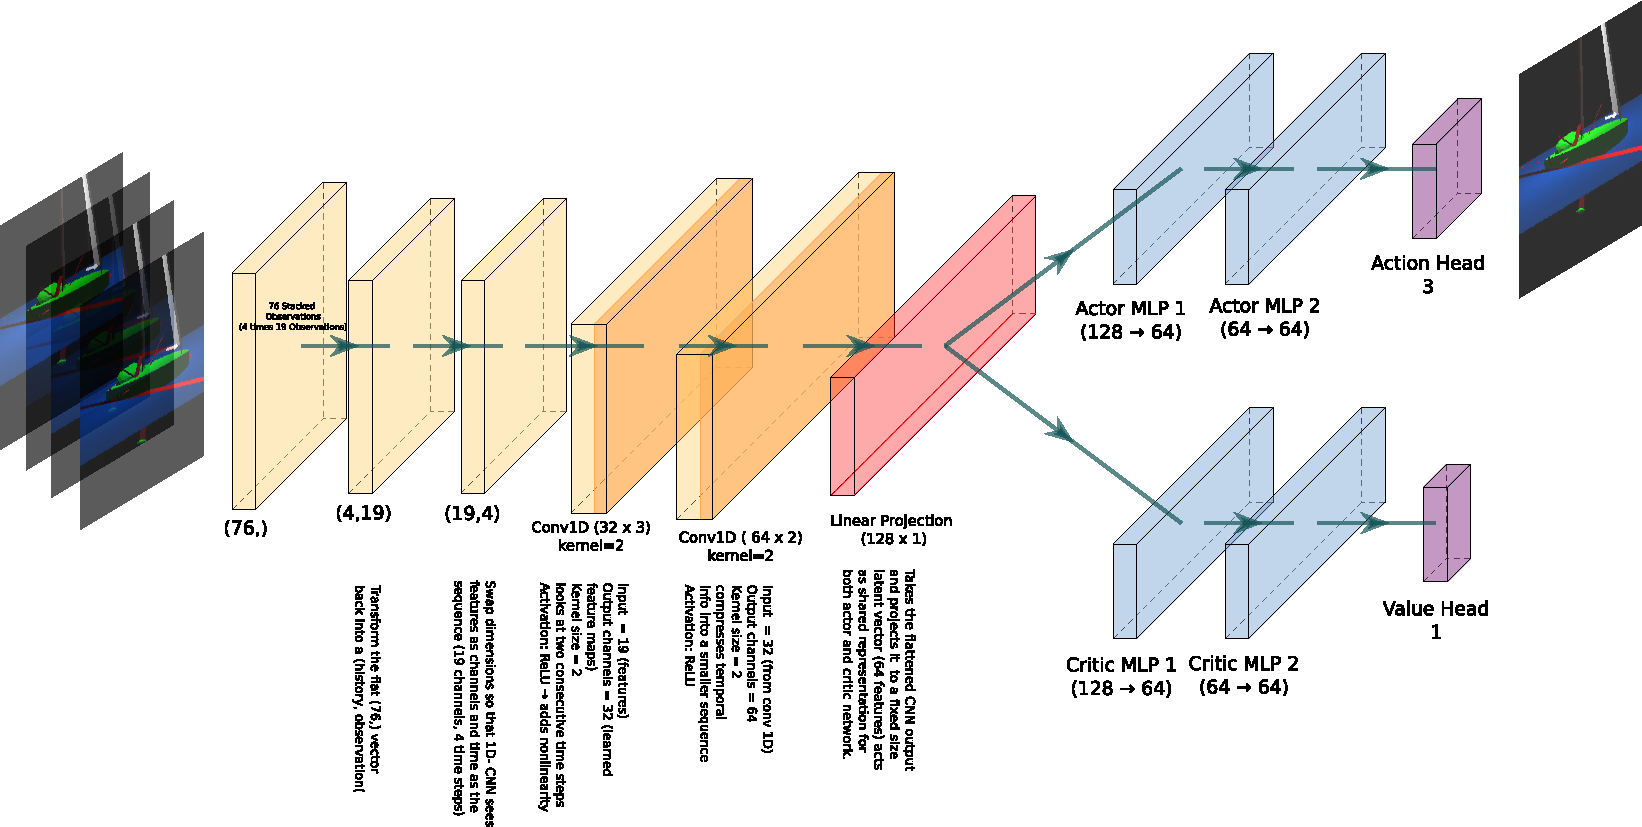
\includegraphics[width=1.0\linewidth]{resources/img/chapter3/1dcnn.pdf}
    \caption{Proposed PPO Actor-Critic network featuring a history-based 1D-CNN feature extractor. The input comprises a temporal stack of 4 consecutive observations ($\sum_{i=0}^{3} \mathbf{o}_{t-i}$). With each observation vector containing 19 physical features, the resulting 76-dimensional input is reshaped into a $(19 \text{ channels} \times 4 \text{ time steps})$ tensor. The CNN architecture employs two Conv1D layers to extract temporal patterns, which are then projected into a 64-dimensional latent representation. This embedding is shared by the Actor and Critic MLP branches to determine the optimal 3D action vector and scalar state value, respectively.}
    \label{fig:1dcnn}
\end{figure}
To address the limitations of the reactive MLP, we introduce the \textbf{HistoryCNNExtractor}, a 1D Convolutional Neural Network (1DCNN) designed to capture temporal dependencies in sailboat (see Figure \ref{fig:1dcnn}). By using a \texttt{VecFrameStack} of $n=4$ frames, the agent receives a rolling history of the environment rather than isolated snapshots. The stacked observations from the last four timesteps, $\sum_{i=1}^{4} \mathbf{o}_{t-i}$, are reshaped so that the 19 physical features are treated as channels and the four steps form the temporal dimension. This allows the convolutional kernels to slide along the time axis while observing all sensor features simultaneously at each temporal position.  

Physically, the 1D-CNN functions as a \textit{learnable differential operator}. The first convolutional layer, with a kernel size of 2, is mathematically analogous to a first-order difference operator in time:
\[
\Delta x_t = x_t - x_{t-1}.
\]
This allows the network to detect temporal trends such as the onset of wind gusts or sustained shifts in direction, providing the agent with richer information for anticipatory decision-making that improves CMG and overall sailing performance.

\begin{figure}[H]
    \centering
    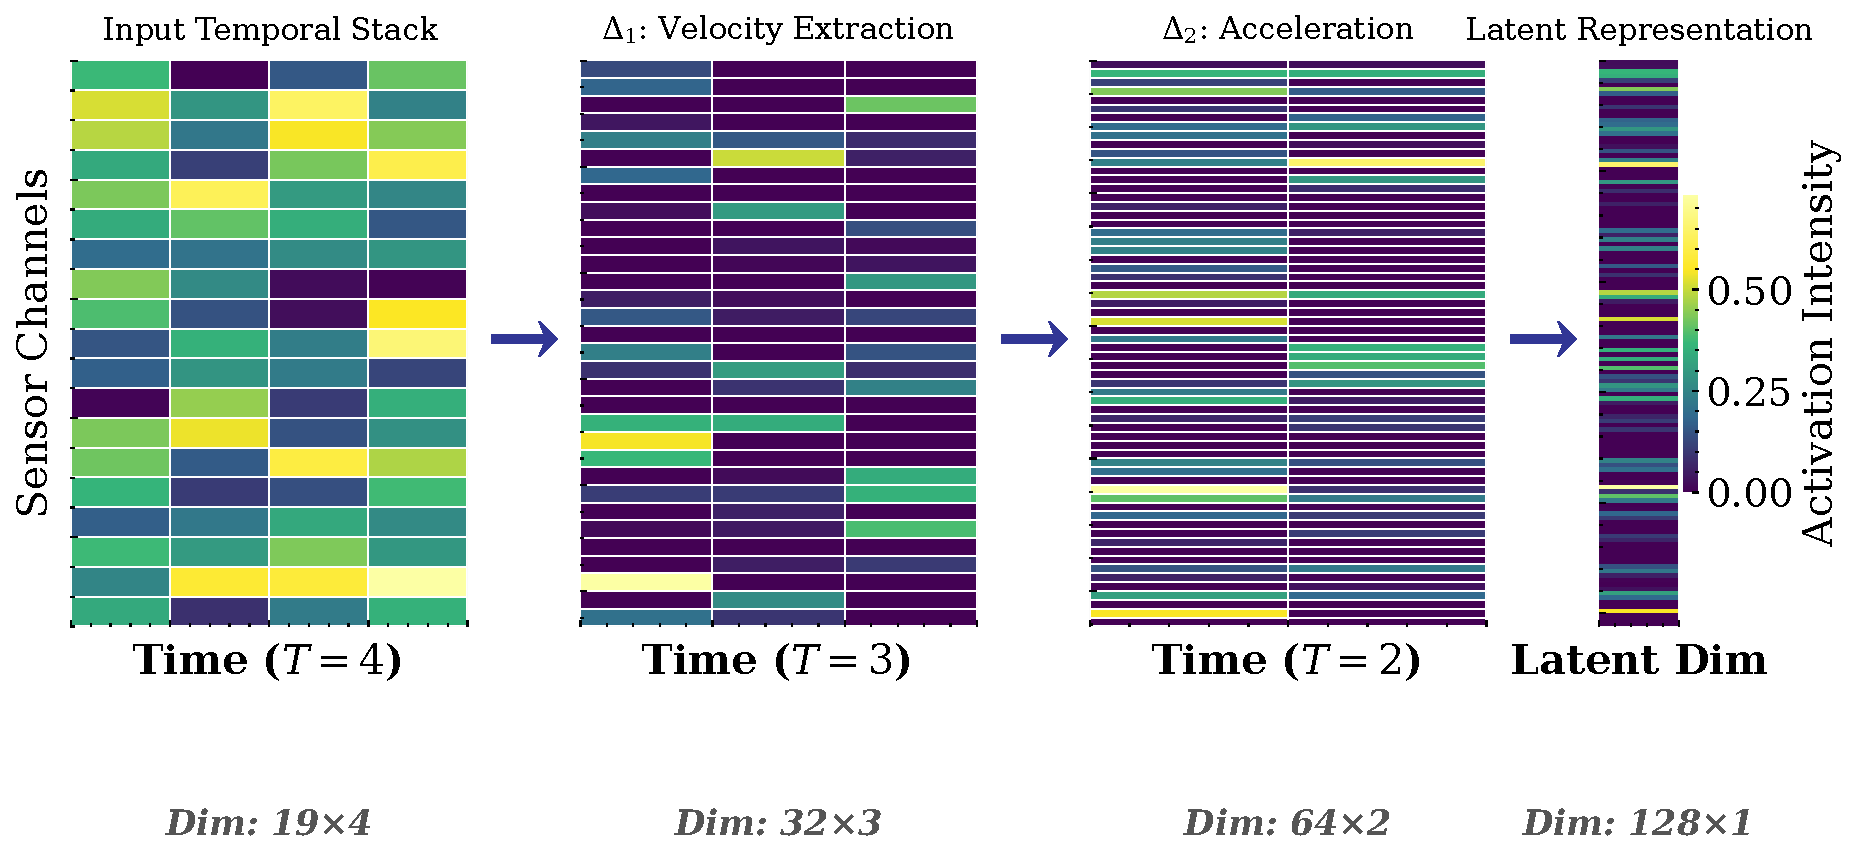
\includegraphics[width=1\linewidth]{resources/img/chapter3/dataflow_1dcnn.pdf}
    \caption{Hierarchical dataflow through the 1D-CNN feature extractor. \textbf{Panel 1:} Raw input matrix ($19 \text{ features} \times 4 \text{ steps}$). \textbf{Panel 2:} After the first convolution ($k=2$), the temporal dimension is reduced to 3; the 32 feature channels act as first-order differential operators. \textbf{Panel 3:} The second convolution reduces the temporal window to 2, processing velocity signals to extract second-order dynamics (acceleration). \textbf{Panel 4:} The latent representation, flattened to $64 \text{ channels} \times 2 \text{ steps} = 128$, provides a high-level physical abstraction for the Actor-Critic heads.}
    \label{fig:dataflow}
\end{figure}

The network autonomously extracts \emph{velocity-like} features, such as the rate of change in wind angle or boat speed. The second convolutional layer captures higher-order differences, effectively computing \emph{acceleration-like} features. With a temporal window of four frames, the network achieves sufficient depth to stabilize these derivatives against simulation noise and environmental stochasticity. The resulting high-level features are flattened into a 128-dimensional latent embedding, which is passed to the Actor-Critic heads, providing a time-aware representation of the vessel’s momentum and trajectory. As illustrated in Figure \ref{fig:dataflow}, this architecture enables the agent to go beyond reactive control, making proactive navigation decisions informed by evolving environmental trends.


\subsection{Training Protocol}
Each training episode was limited to a maximum of 512 steps, with a control frequency of $2\,\text{Hz}$ (the agent produced control decisions every 0.5 seconds). The action space is a discrete space allowing the agent to make incremental adjustments to the desired course (turn left, turn right, or maintain heading). Training was conducted under randomized environmental conditions to promote robustness and generalization. Wind speed was sampled uniformly between 10 and 18 knots, while target headings were drawn from upwind and reaching\footnote{wind comes from the side of the boat} configurations ranging from $90^\circ$ to $140^\circ$ relative to the true wind direction. Navigation precision was enforced through a narrow target definition consisting of an $8^\circ$ bearing width and a 1\,m positional tolerance, encouraging accurate trajectory tracking.

\subsubsection{Reward Design: CMG Optimization Objective}

The primary learning objective was to maximize CMG. The reward function was defined as:
\[
R = V_{\text{boat}} \cdot \cos(\theta_{\text{error})}
\]
where $V_{\text{boat}} \cdot \cos(\theta_{\text{error}})$ represents the component of velocity aligned with the target direction. The term $C_{\text{oob}}$ corresponds to a significant penalty (50 units) applied when the sailboat exits operational boundaries or loses foil stability, while $C_{\text{heading}}$ enforces a maximum deviation constraint of $45^\circ$ from the target heading.

This reward structure encourages sustained high-speed motion while maintaining directional accuracy and stable foiling behaviour.


